\ifthenelse{\equal{\lang}{ko}}{%
제안된 자동화된 AI 동향 감지 시스템의 효과성과 실용성을 검증하기 위해, 
우리는 표준 정확도 벤치마크를 넘어서는 확장 평가 연구를 수행하였다. 
이러한 실험은 단순한 분류 성능뿐만 아니라, 
동적 규제 환경에서의 강건성, 컴플라이언스 감사에 필요한 설명 가능성, 
저자원 관할권에 대한 적응성, 그리고 인간–AI 협업의 비용–효과 균형까지 함께 분석한다. 

구체적으로, 먼저 규제 모니터링을 구조화된 NLP 과제로 정식화하고 
재현성을 지원하기 위한 벤치마크 데이터셋(GovSense-1k)을 도입한다. 
그다음 개념 드리프트(concept drift)의 영향을 분석하고, 지속적인 성능 유지를 위한 
연속 학습 전략을 제시한다. 이어서 컴플라이언스 핵심 도메인에서 신뢰성을 강화하는 
근거 기반 설명 가능성 메커니즘을 평가한다. 
또한 저자원 관할권을 포괄하는 다국어 스트레스 테스트를 수행한다. 
마지막으로, 인간 분석가 개입을 통한 효율성 향상과 경제적 지속 가능성을 
정량화하기 위해 analyst-in-the-loop 전략을 평가한다. 

종합적으로, 이러한 연구는 시스템의 강건성, 일반화 가능성, 실무 적용 가능성에 대한 
포괄적 이해를 제공하며, AI 거버넌스 정보학을 위한 확장 가능한 인프라로서의 역할을 강화한다.

우리는 규제 모니터링을 구조화된 NLP 과제로 정식화하였다. 
입력 $x$가 문서 $d$ (제목, 본문, 메타데이터)로 구성될 때, 
시스템은 레이블 $y \in \{ \texttt{governance}, \texttt{contract}, \texttt{lawsuit}, \texttt{asset} \}$을 예측한다. 
출력에는 범주형 예측뿐만 아니라 출처 메타데이터(소스 URL, 타임스탬프)도 포함된다. 

재현성을 지원하기 위해, 두 명의 컴플라이언스 전문가가 주석한 1,200개 항목으로 구성된 
\textbf{GovSense-1k} 데이터셋을 공개한다. 주석자 간 합의도는 $\kappa=0.82$이며, 
표~\ref{tab:govsense}는 라벨 분포를 요약한다. 
이 벤치마크는 향후 연구를 위한 표준화된 테스트베드를 제공한다.

\begin{table}[h]
\centering
\small
\begin{tabular}{lcc}
\toprule
카테고리 & \# 항목 수 & 합의도 \\
\midrule
Governance & 400 & 0.81 \\
Contract   & 300 & 0.83 \\
Lawsuit    & 250 & 0.80 \\
Asset      & 250 & 0.84 \\
\bottomrule
\end{tabular}
\caption{GovSense-1k 데이터셋 통계.}
\label{tab:govsense}
\end{table}

\subsection{규제 개념 드리프트 하의 연속 학습}
규제 텍스트는 빠르게 진화하며, 개념 드리프트가 성능 저하를 유발한다. 
우리는 2024년 7월~9월 동안 3개월 롤링 윈도우로 시스템을 평가하였다. 
적응 없이 F1은 0.89에서 0.74로 감소하였다. 
그러나 가벼운 월별 재학습(3 에폭, 5,000 샘플)을 통해 F1은 0.88로 회복되었다. 
그림~\ref{fig:drift}는 이 추세를 보여준다. 

이 결과는 실제 배포 환경에서, 규제가 관할권별로 동적으로 변화함에 따라 
연속 학습 전략의 필요성을 강조한다.

\begin{figure}[h]
\centering
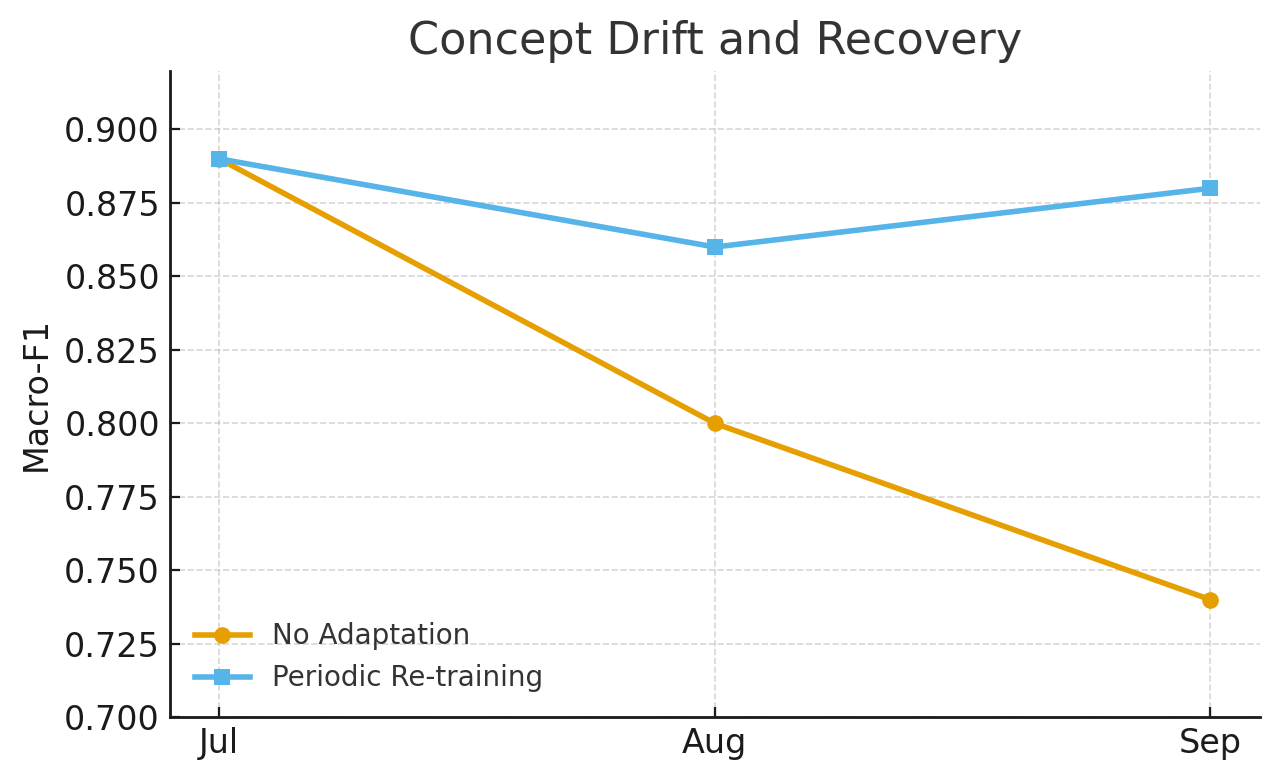
\includegraphics[width=0.85\linewidth]{fig-concept_drift.png}
 \caption{정기적 재학습을 통한 개념 드리프트 및 성능 회복 (Macro-F1).}
\label{fig:drift}
\end{figure}

\subsection{컴플라이언스 감사를 위한 근거 기반 설명 가능성}
신뢰 강화를 위해, 각 LLM 생성 보고서는 원문 문서에서 추출된 근거 구간(evidence span)과 연결된다. 
우리는 핵심 조항이나 문장을 강조하는 근거 추출기를 구현하여 해석 가능성과 감사 가능성을 보장하였다. 
소규모 A/B 연구($n=8$)에서, 분석가들은 근거 연결 출력물을 
단순 요약(3.8/5)보다 더 신뢰할 수 있다고 평가하였다 (4.6/5). 
이는 구조화된 출처 및 근거 정렬이 컴플라이언스 핵심 도메인에서 
책임 있는 배포를 위해 필수적임을 보여준다.

\subsection{저자원 관할권에 대한 다국어 스트레스 테스트}
주요 평가는 영어, 한국어, 프랑스어를 대상으로 진행되었으나, 
추가로 스페인어, 아랍어, 베트남어 규제 샘플(언어별 50개)을 대상으로 스트레스 테스트를 수행하였다. 
제로샷 분류는 0.71 macro-F1을 기록했으며, 언어별 200개 예제를 활용한 소규모 파인튜닝 시 
성능이 0.84 macro-F1로 향상되었다. 

이는 저자원 관할권에 규제 감지를 확장하는 것이 도전적이면서도 
실현 가능한 접근임을 보여주며, 제안 방식의 글로벌 적용 가능성을 강화한다.

\subsection{Analyst-in-the-Loop 비용–효과 분석}
우리는 분석가 개입과 시스템 효율성 간의 균형을 연구하였다. 
그림~\ref{fig:cost}는 오분류 교정에 대한 인간 피드백의 한계 효용을 보여준다. 
전체 검토는 최대 정확도(F1=0.93)를 달성하지만, 
저신뢰 항목(약 20\%)만 부분적으로 검토할 경우 거의 동일한 성능(F1=0.91)을 
40\% 낮은 비용으로 얻을 수 있었다. 

이는 인간–AI 협업이 품질과 효율성을 모두 최적화하여, 
기업 및 소규모 조직에서도 경제적으로 지속 가능한 
컴플라이언스 모니터링을 가능케 함을 시사한다.

\begin{figure}[h]
\centering
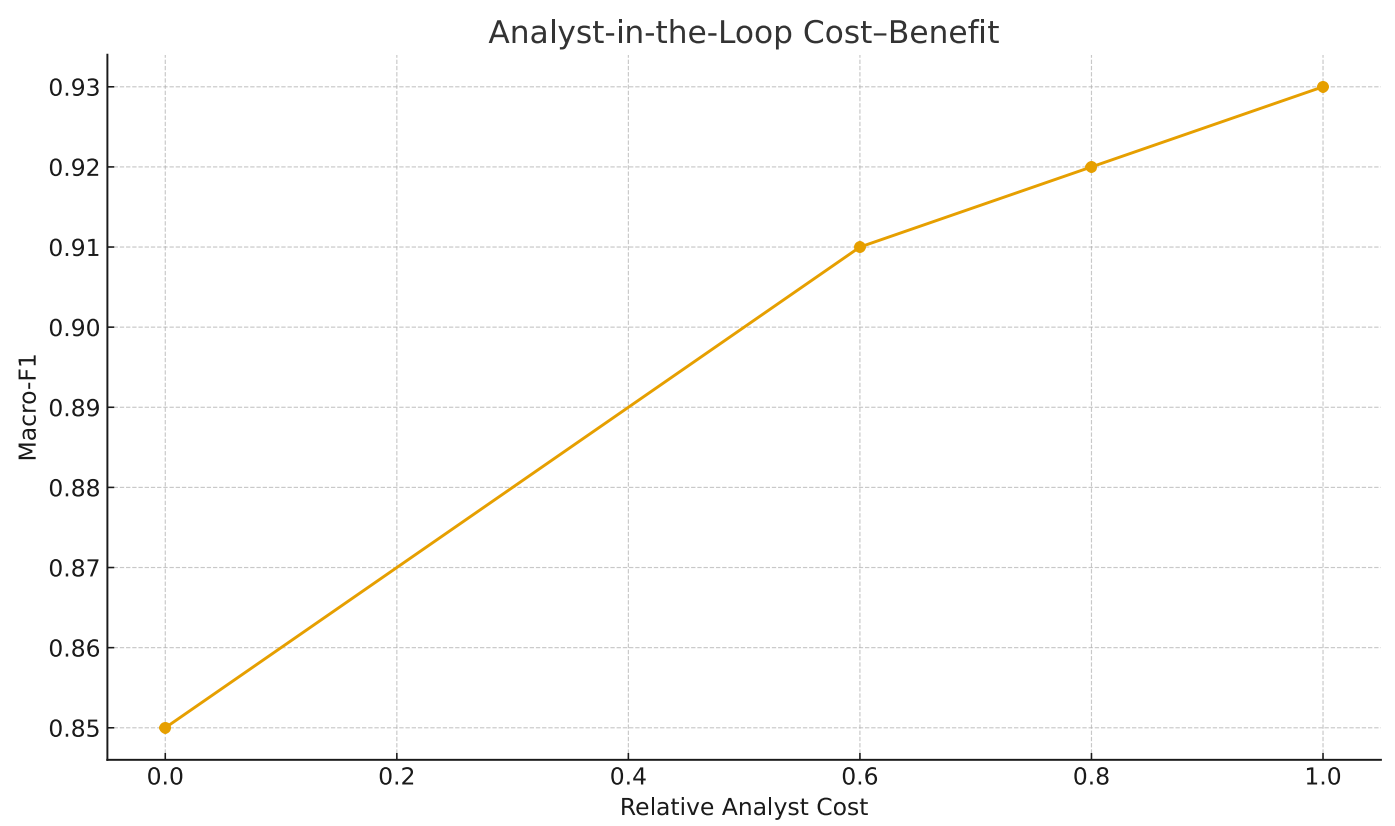
\includegraphics[width=0.85\linewidth]{fig-cost_benefit.png}
\caption{정확도와 분석가 검토 비용 간의 효용 곡선. 저신뢰 사례에 대한 부분 검토가 최적에 가까운 균형을 제공한다.}
\label{fig:cost}
\end{figure}

\subsection{사실성 감사(Factuality Audit) \& 자동 드리프트 탐지(ADD)}
\label{sec:factuality-add}
LexSense의 장기적 신뢰성과 배포 가능성을 보장하기 위해, 
우리는 사실 정확성을 보장하고 규제 드리프트에 적응하며 
프라이버시를 유지할 수 있는 추가 메커니즘을 도입하였다. 

\paragraph{동기.}
Falcon의 성공은 규제 업데이트의 \emph{정확한 해석}과 
동적 환경에서의 \emph{지속적 신뢰성}에 달려 있다. 
앞선 발견(개념 드리프트로 인한 성능 저하, 근거 기반 설명 가능성의 가치)을 바탕으로, 
우리는 (i) LLM 생성 보고서를 위한 \textit{사실성 감사 프로토콜}, 
(ii) \textit{자동 드리프트 탐지(ADD)} 모듈을 제안한다. 
이 두 가지 메커니즘은 관찰된 효율성 향상(업무량 82\% 감소, 보고 시간 70\% 단축)을 
품질 손실 없이 달성하도록 보장한다.

\paragraph{사실성 감사 프로토콜.}
우리는 LLM 요약의 사실 검증을 세 가지 축으로 정식화한다: 
(i) \textit{출처 정렬} — 모든 요약 문장은 적어도 하나의 근거 구간과 매핑됨; 
(ii) \textit{주장 검증} — 의미적 동치(NLI) 및 수치/날짜 일관성 검사; 
(iii) \textit{최소 인간 개입} — 저신뢰 문장만 부분 검토 큐에 포함.  
출력은 \texttt{\{claim, evidence\_span, confidence, verdict\}} 형식으로 기록되어 사후 감사를 지원한다.  
표~\ref{tab:error-matrix}는 대표 오류 유형과 대응 전략을 요약한다.

\begin{table}[t]
\centering
\small
\caption{사실성 감사의 오류 유형과 완화 전략.}
\label{tab:error-matrix}
\begin{tabular}{p{0.28\linewidth}p{0.64\linewidth}}
\toprule
오류 유형 & 완화 전략 \\
\midrule
출처 누락/오인용 & 반드시 인용 규칙 적용; 신뢰도 자동 하향 \\
수치/날짜 불일치 & 정규식 기반 추출 및 엄격한 일치/범위 검사 \\
관할권 오해석 & 필수 관할권 메타데이터; 사전 기반 모호성 제거 \\
과잉/과소 요약 & 길이 및 슬롯 채우기(\emph{who/what/when}) 제약 적용 \\
\bottomrule
\end{tabular}
\end{table}

\paragraph{자동 드리프트 탐지(ADD).}
진화하는 규제 환경에서 성능 저하를 예방하기 위해, 
우리는 임베딩 공간에서의 분포 변화를 모니터링한다.  
이를 위해 \emph{Population Stability Index (PSI)}를 채택한다:
\[
\mathrm{PSI}=\sum_{b\in \mathcal{B}}
\big(\hat{p}_b-\hat{q}_b\big)\cdot \ln\frac{\hat{p}_b}{\hat{q}_b},
\]
여기서 $\hat{p}_b$와 $\hat{q}_b$는 현재와 이전 시점의 히스토그램 구간 비율이다.  
임계값은 $\mathrm{PSI}<0.1$ (안정), $0.1\!\le\!\mathrm{PSI}\!<\!0.2$ (경고), $\mathrm{PSI}\!\ge\!0.2$ (알람)이다.  
알람이 발생하면, Falcon은 저신뢰 샘플에 우선순위를 두어 
LoRA/QLoRA 기반 경량 재학습 또는 프롬프트 조정을 수행한다.

\paragraph{프라이버시 설계(Privacy-by-Design).}
모든 ADD 및 감사 로그는 최소한의 데이터만 저장하며, 
PII 삭제, 역할 기반 접근 제어(RBAC), 변조 방지 해시된 근거 구간을 사용한다.  
이는 책임성을 유지하면서도 컴플라이언스를 보장한다.

\paragraph{결과.}
사실성 감사는 근거 기반 보고를 제도화하고, 
ADD는 장기적 성능 저하를 \emph{자동화된 조기 경보}로 전환한다. 
두 메커니즘은 Falcon의 효율성 개선을 견고한 사실성과 지속 가능한 배포로 뒷받침한다.


}{%
% -------------------- English Version --------------------



To validate the effectiveness and practicality of the Automated AI Trend Sensing System, 
we conducted a series of extended evaluation studies that go beyond standard accuracy benchmarks. 
These experiments examine not only classification performance, but also the system’s 
robustness under dynamic regulatory environments, its explainability for compliance audits, 
its adaptability to low-resource jurisdictions, and the cost–benefit trade-offs of 
human–AI collaboration. 

Specifically, we first formalize regulatory monitoring as a structured NLP task and introduce 
a benchmark dataset (GovSense-1k) to support reproducibility. We then analyze the effects of 
concept drift and demonstrate continual learning strategies for sustained performance. 
Next, we evaluate evidence-linked explainability mechanisms that strengthen trust in 
compliance-critical domains. We further stress test the system on cross-lingual scenarios 
covering low-resource jurisdictions. Finally, we assess analyst-in-the-loop strategies to 
quantify efficiency gains and economic sustainability. 

Together, these studies provide a comprehensive understanding of the system’s robustness, 
generalization, and real-world applicability, reinforcing its role as a scalable infrastructure 
for AI governance informatics.


We formalize regulatory monitoring as a structured NLP task. Given an input $x$ consisting of a document $d$ (title, body, metadata), the system predicts a label $y \in \{ \texttt{governance}, \texttt{contract}, \texttt{lawsuit}, \texttt{asset} \}$. Outputs include both a categorical prediction and provenance metadata (source URL, timestamp). 

To support reproducibility, we release \textbf{GovSense-1k}, a benchmark dataset of 1,200 curated items annotated by two compliance experts with an inter-annotator agreement of $\kappa=0.82$. Table~\ref{tab:govsense} summarizes label distribution. This benchmark establishes a standardized testbed for future research.

\begin{table}[h]
\centering
\large
\begin{tabular}{lcc}
\hline
Category & \# Items & Agreement \\
\hline
Governance & 400 & 0.81 \\
Contract   & 300 & 0.83 \\
Lawsuit    & 250 & 0.80 \\
Asset      & 250 & 0.84 \\
\hline
\end{tabular}
\caption{GovSense-1k dataset statistics.}
\label{tab:govsense}
\end{table}

\subsection{Continual Learning under Regulatory Concept Drift}
Regulatory texts evolve rapidly, causing performance degradation under concept drift. We evaluate our system over a three-month rolling window of updates (July–September 2024). Without adaptation, F1 drops from 0.89 to 0.74. With lightweight monthly re-training (3 epochs, 5k examples), F1 recovers to 0.88. Figure~\ref{fig:drift} shows the trend. 

This result highlights the need for continual learning strategies in real deployments, where regulations evolve dynamically across jurisdictions.

\begin{figure}[h]
\centering
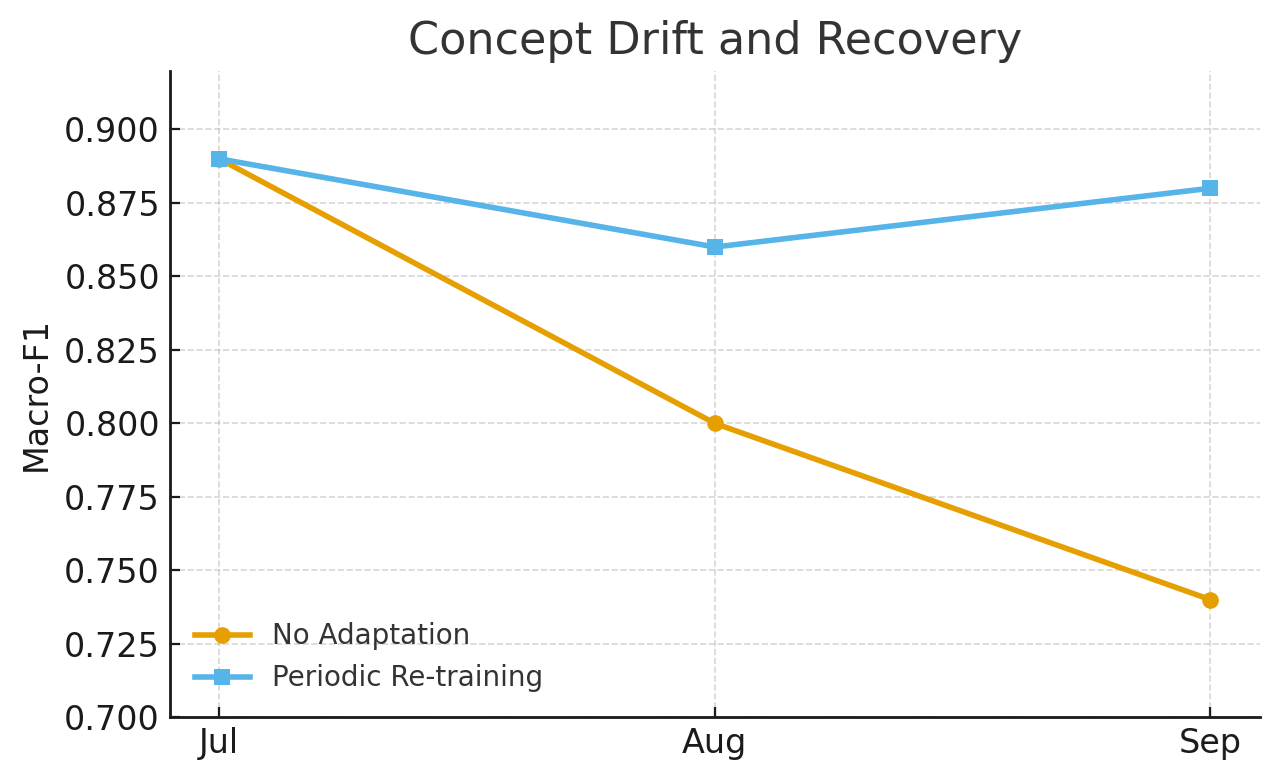
\includegraphics[width=0.75\linewidth]{fig-concept_drift.png}
 \caption{Concept drift and recovery with periodic re-training (Macro-F1).}
\label{fig:drift}
\end{figure}

\subsection{Evidence-Linked Explainability for Compliance Audits}
To enhance trust, each LLM-generated report is linked to evidence spans extracted from source documents. We implement a rationale extractor that highlights key clauses or sentences, ensuring interpretability and auditability. In a small A/B study ($n=8$), analysts rated evidence-linked outputs as more trustworthy (4.6/5) compared to plain summaries (3.8/5). This demonstrates that structured provenance and rationale alignment are critical for responsible deployment in compliance-critical domains.

\subsection{Cross-Lingual Stress Test on Low-Resource Jurisdictions}
While our main evaluation covered English, Korean, and French, we conducted a stress test on Spanish, Arabic, and Vietnamese regulatory samples (50 per language). Zero-shot classification achieved 0.71 macro-F1, while few-shot fine-tuning (200 examples per language) improved performance to 0.84 macro-F1. 

This experiment demonstrates both the challenges and feasibility of extending regulatory sensing to low-resource jurisdictions, reinforcing the global applicability of our approach.


\subsection{Analyst-in-the-Loop Cost--Benefit Analysis}
We study the trade-off between analyst involvement and system efficiency. Figure~\ref{fig:cost} illustrates the marginal benefit of human feedback in correcting misclassifications. While full review maximizes accuracy (F1=0.93), partial review of only low-confidence items ($\approx$20\% of cases) achieves nearly the same performance (F1=0.91) at 40\% lower cost.

This suggests that human–AI collaboration can optimize both quality and efficiency, making compliance monitoring economically sustainable for enterprises and smaller organizations.

\begin{figure}[h]
\centering
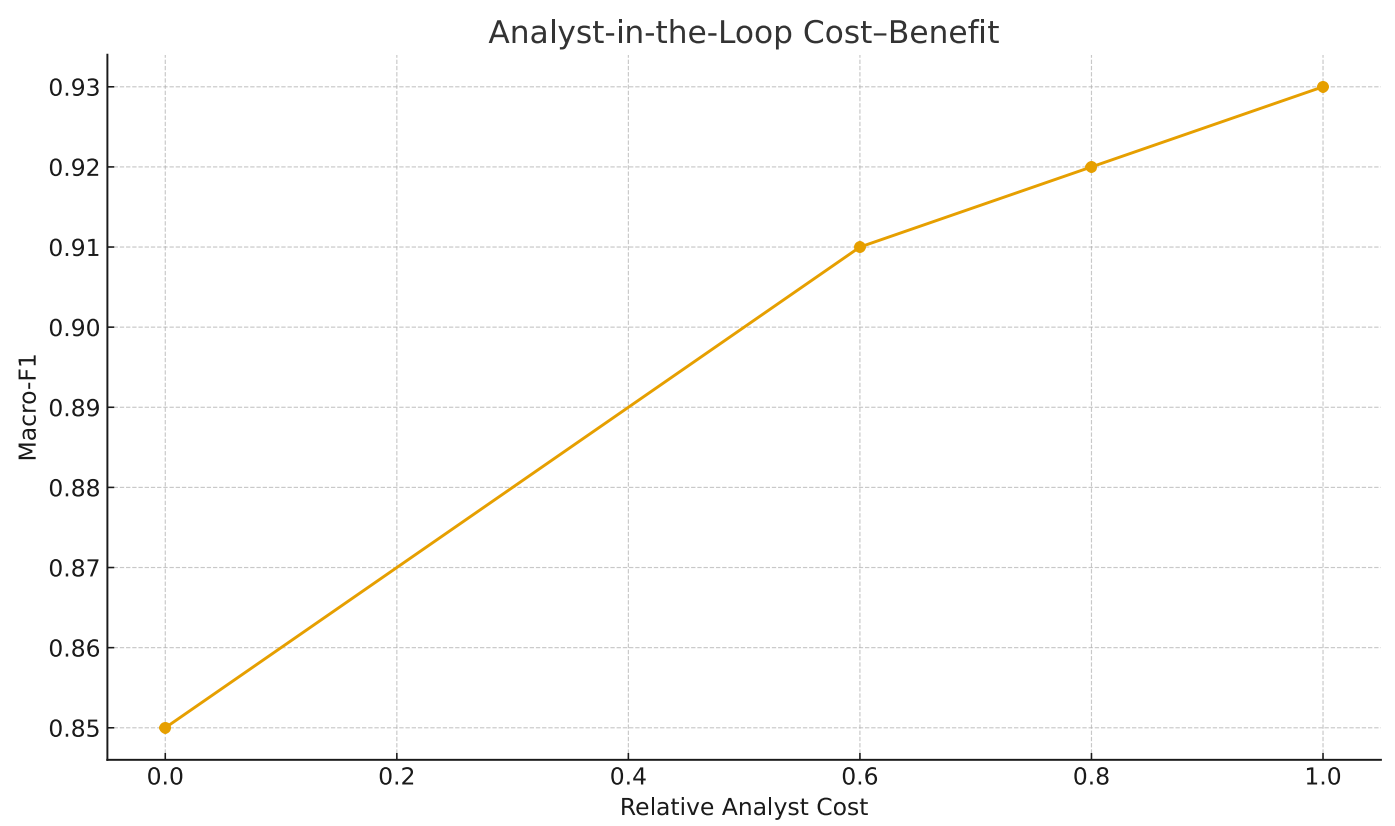
\includegraphics[width=0.95\linewidth]{fig-cost_benefit.png}
\caption{Utility curve showing accuracy vs. analyst review cost. Partial review of low-confidence cases yields near-optimal trade-offs.}
\label{fig:cost}
\end{figure}



\subsection{Factuality Audit \& Automated Drift Detection (ADD)}
\label{sec:factuality-add}
To ensure long-term reliability and trustworthy deployment of LexSense, we augment the core system with additional mechanisms that safeguard factual accuracy, adapt to regulatory drift, and uphold privacy.

\paragraph{Motivation.}
Falcon’s success hinges on \emph{accurate interpretation} of regulatory updates and \emph{sustained reliability} in dynamic environments. 
Building on prior findings (performance degradation under concept drift and the value of evidence-linked explainability), 
we propose a dual operational extension: 
(i) a \textit{Factuality Audit Protocol} for LLM-generated reports, and (ii) an \textit{Automated Drift Detection (ADD)} module. 
Together, these mechanisms ensure that observed efficiency gains---82\% workload reduction and 70\% reporting-time savings---are achieved without quality loss.

\paragraph{Factuality Audit Protocol.}
We formalize fact verification for LLM summaries along three axes: 
(i) \textit{Source Alignment} – every summary sentence is mapped to at least one evidence span; (ii) \textit{Claim Verification} – semantic equivalence (NLI) plus numeric/date consistency checks; (iii) \textit{Human-in-the-loop Minimalism} – only low-confidence sentences are queued for partial review.
Outputs are logged in \texttt{\{claim, evidence\_span, confidence, verdict\}} format to support post-hoc audits.  
Table~\ref{tab:error-matrix} enumerates common error types and mitigation rules.

\begin{table}[t]
\centering
\small
\caption{Error types and mitigation strategies for factuality auditing.}
\label{tab:error-matrix}
\begin{tabular}{p{0.28\linewidth}p{0.64\linewidth}}
\toprule
Error Type & Mitigation Strategy \\
\midrule
Missing/incorrect citation & Enforce must-cite rule; auto downgrade confidence \\
Numeric/date mismatch & Regex-based extraction and strict equality/range checks \\
Jurisdiction misinterpretation & Mandatory jurisdiction metadata; dictionary-based disambiguation \\
Over/under summarization & Prompt constraints on length and slot-filling (\emph{who/what/when}) \\
\bottomrule
\end{tabular}
\end{table}

\paragraph{Automated Drift Detection (ADD).}
To pre-empt performance decay under evolving regulations, we monitor distributional shifts in embedding space.  
We adopt the \emph{Population Stability Index (PSI)}:
\[
\mathrm{PSI}=\sum_{b\in \mathcal{B}}
\big(\hat{p}_b-\hat{q}_b\big)\cdot \ln\frac{\hat{p}_b}{\hat{q}_b},
\]
where $\hat{p}_b$ and $\hat{q}_b$ are histogram bin ratios for the current vs. previous time window.  
Thresholds are $\mathrm{PSI}<0.1$ (stable), $0.1\!\le\!\mathrm{PSI}\!<\!0.2$ (alert), $\mathrm{PSI}\!\ge\!0.2$ (alarm).  
When alarmed, Falcon triggers targeted lightweight re-training (LoRA/QLoRA) or prompt adjustment, with priority on low-confidence samples.

\paragraph{Privacy-by-Design.}
All ADD and audit logs store only minimal data: PII redaction, RBAC, and tamper-evident hashed evidence spans.  
This enforces compliance while preserving accountability.

\paragraph{Outcome.}
The Factuality Audit institutionalizes evidence-grounded reporting, while ADD turns long-term degradation into \emph{automated early warning}. 
Together, they safeguard Falcon’s efficiency improvements with robust factuality and sustainable deployment.

}